\chapter{The Perceptron} \label{sec:perc}

\chapterquote{Algebra is nothing more than geometry, in words; geometry is nothing more than algebra, in pictures.}{Sophie~Germain}


\begin{learningobjectives}
\item Describe the biological motivation behind the perceptron.
\item Classify learning algorithms based on whether they are
  error-driven or not.
\item Implement the perceptron algorithm for binary classification.
\item Draw perceptron weight vectors and the corresponding decision
  boundaries in two dimensions.
%\item Define linear separability, and be able to turn any arbitrary
%  data set into a linearly separable data set.
\item Contrast the decision boundaries of decision trees, nearest
  neighbor algorithms and perceptrons.
\item Compute the margin of a given weight vector on a given data set.
\end{learningobjectives}

\dependencies{\chref{sec:dt}, \chref{sec:knn}}

\newthought{So far, you've seen two types} of learning models: in
decision trees, only a small number of features are used to make
decisions; in nearest neighbor algorithms, all features are used
equally.  Neither of these extremes is always desirable.  In some
problems, we might want to use most of the features, but use some more
than others.

In this chapter, we'll discuss the \concept{perceptron} algorithm for
learning \concept{weights} for features.  As we'll see, learning
weights for features amounts to learning a \concept{hyperplane}
classifier: that is, basically a division of space into two halves by
a straight line, where one half is ``positive'' and one half is
``negative.''  In this sense, the perceptron can be seen as explicitly
finding a good \concept{linear decision boundary}.

\section{Bio-inspired Learning}

\Figure{perc:neuron}{a picture of a neuron}

Folk biology tells us that our brains are made up of a bunch of little
units, called \concept{neurons}, that send electrical signals to one
another.  The \emph{rate} of firing tells us how ``activated'' a
neuron is.  A single neuron, like that shown in
Figure~\ref{fig:perc:neuron} might have three incoming neurons.  These
incoming neurons are firing at different rates (i.e., have different
\concept{activations}).  Based on how much these incoming neurons are
firing, and how ``strong'' the neural connections are, our main neuron
will ``decide'' how strongly it wants to fire.  And so on through the
whole brain.  Learning in the brain happens by neurons becomming
connected to other neurons, and the strengths of connections adapting
over time.

\Figure{perc:example}{figure showing feature vector and weight
  vector and products and sum}

The real biological world is much more complicated than this.
However, our goal isn't to build a brain, but to simply be
\emph{inspired} by how they work.  We are going to think of our
learning algorithm as a \emph{single} neuron.  It receives input from
$D$-many other neurons, one for each input feature.  The strength of
these inputs are the feature values.  This is shown schematically in
Figure~\ref{fig:perc:neuron}.  Each incoming connection has a weight
and the neuron simply sums up all the weighted inputs.  Based on this
sum, it decides whether to ``fire'' or not.  Firing is interpreted as
being a positive example and not firing is interpreted as being a
negative example.  In particular, if the weighted sum is positive, it
``fires'' and otherwise it doesn't fire.  This is shown
diagramatically in Figure~\ref{fig:perc:example}.

Mathematically, an input vector $\vx = \langle x_1, x_2, \dots, x_D
\rangle$ arrives.  The neuron stores $D$-many weights, $w_1, w_2,
\dots, w_D$.  The neuron computes the sum:
\begin{equation} \label{eq:perc:sum}
a = \sum_{d=1}^D w_d x_d
\end{equation}
to determine it's amount of ``activation.''  If this activiation is
positive (i.e., $a > 0$) it predicts that this example is a positive
example.  Otherwise it predicts a negative example.

The weights of this neuron are fairly easy to interpret.  Suppose that
a feature, for instance ``is this a System's class?'' gets a zero
weight.  Then the activation is the same regardless of the value of
this feature.  So features with zero weight are ignored.  Features
with positive weights are indicative of positive examples because they
cause the activation to increase.  Features with negative weights are
indicative of negative examples because they cause the activiation to
decrease.

\thinkaboutit{What would happen if we encoded binary features like
  ``is this a System's class'' as no=$0$ and yes=$-1$ (rather than the
  standard no=$0$ and yes=$+1$)?}

It is often convenient to have a non-zero \concept{threshold}.  In
other words, we might want to predict positive if $a > \th$ for some
value $\th$.  The way that is most convenient to achieve this is to
introduce a \concept{bias} term into the neuron, so that the
activation is always increased by some fixed value $b$.  Thus, we
compute:
\begin{equation} \label{eq:perc:sumbias}
a = \left[ \sum_{d=1}^D w_d x_d \right] + b
\end{equation}
\thinkaboutit{If you wanted the activation threshold to be $a > \th$
  instead of $a > 0$, what value would $b$ have to be?}

This is the complete neural model of learning.  The model is
parameterized by $D$-many weights, $w_1, w_2, \dots, w_D$, and a
single scalar bias value $b$.

\section{Error-Driven Updating: The Perceptron Algorithm}

The \concept{perceptron} is a classic learning algorithm for the
neural model of learning.  Like $K$-nearest neighbors, it is one of
those frustrating algorithms that is incredibly simple and yet works
amazingly well, for some types of problems.

The algorithm is actually quite different than either the decision
tree algorithm or the KNN algorithm.  First, it is \concept{online}.
This means that instead of considering the \emph{entire data set} at
the same time, it only ever looks at one example.  It processes that
example and then goes on to the next one.  Second, it is
\concept{error driven}.  This means that, so long as it is doing well,
it doesn't bother updating its parameters.

The algorithm maintains a ``guess'' at good parameters (weights and
bias) as it runs.  It processes one example at a time.  For a given
example, it makes a prediction.  It checks to see if this prediction
is correct (recall that this is \emph{training data}, so we have
access to true labels).  If the prediction is correct, it does
nothing.  Only when the prediction is incorrect does it change its
parameters, and it changes them in such a way that it would do better
on this example next time around.  It then goes on to the next
example.  Once it hits the last example in the training set, it loops
back around for a specified number of iterations.

\newalgorithm%
  {perc:perc}%
  {\FUN{PerceptronTrain}(\VAR{$\mat D$}, \VAR{MaxIter})}
  {
\SETST{$w_d$}{\CON{0}, \text{for all } \VAR{$d$} = $\CON{1} \dots \VAR{D}$}
  \COMMENT{initialize weights}
\SETST{$b$}{\CON{0}}
  \COMMENT{initialize bias}
\FOR{\VAR{iter} = \CON{1} \dots \VAR{MaxIter}}
\FORALL{(\VAR{$\vx$},\VAR{$y$}) $\in$ \VAR{$\mat D$}}
\SETST{$a$}{$\sum_{\VAR{d}=\CON{1}}^{\VAR{D}}$ \VAR{$w_d$} \VAR{$x_d$} + \VAR{$b$}} 
  \COMMENT{compute activation for this example}
\IF{\VAR{$y$}\VAR{$a$} $\leq \CON{0}$}
\SETST{$w_d$}{\VAR{$w_d$} + \VAR{$y$}\VAR{$x_d$}, \text{for all } \VAR{$d$} = $\CON{1} \dots \VAR{D}$}
  \COMMENT{update weights}
\SETST{$b$}{\VAR{$b$} + \VAR{$y$}}
  \COMMENT{update bias}
\ENDIF
\ENDFOR
\ENDFOR
\RETURN \VAR{$w_0$}, \VAR{$w_1$}, \dots, \VAR{$w_D$}, \VAR{$b$}
}

\newalgorithm%
  {perc:perctest}%
  {\FUN{PerceptronTest}(\VAR{$w_0$}, \VAR{$w_1$}, \dots, \VAR{$w_D$}, \VAR{$b$}, \VAR{$\hat\vx$})}
  {
\SETST{$a$}{$\sum_{\VAR{d}=\CON{1}}^{\VAR{D}}$ \VAR{$w_d$} \VAR{$\hat x_d$} + \VAR{$b$}}
  \COMMENT{compute activation for the test example}
\RETURN \FUN{sign}(\VAR{$a$})
}

The training algorithm for the perceptron is shown in
Algorithm~\ref{alg:perc:perc} and the corresponding prediction
algorithm is shown in Algorithm~\ref{alg:perc:perctest}.  There is one
``trick'' in the training algorithm, which probably seems silly, but
will be useful later.  It is in line 6, when we check to see if we
want to make an update or not.  We want to make an update if the
current prediction (just \FUN{sign}(\VAR{a})) is incorrect.  The trick
is to multiply the true label $y$ by the activation $a$ and compare
this against zero.  Since the label $y$ is either $+1$ or $-1$, you
just need to realize that $ya$ is positive whenever $a$ and $y$ have
the same sign.  In other words, the product $ya$ is positive if the
current prediction is correct.

\thinkaboutit{It is very very important to check $ya
  \leq 0$ rather than $ya < 0$.  Why?}

The particular form of update for the perceptron is quite simple.  The
weight $w_d$ is increased by $y x_d$ and the bias is increased by
$y$.  The goal of the update is to adjust the parameters so that they
are ``better'' for the current example.  In other words, if we saw
this example twice in a row, we should do a better job the second time
around.

To see why this particular update achieves this, consider the
following scenario.  We have some current set of parameters $w_1,
\dots, w_D, b$.  We observe an example $(\vx,y)$.  For simplicity,
suppose this is a positive example, so $y=+1$.  We compute an
activation $a$, and make an error.  Namely, $a<0$.  We now update our
weights and bias.  Let's call the new weights $w'_1, \dots, w'_D,
b'$.  Suppose we observe the same example again and need to compute a
new activation $a'$.  We proceed by a little algebra:
\begin{align}
a'
&= \sum_{d=1}^D w'_d x_d + b' \\
&= \sum_{d=1}^D (\textcolor{darkblue}{w_d} + \textcolor{darkred}{x_d}) x_d + (\textcolor{darkblue}{b} + \textcolor{darkred}{1}) \\
&= \textcolor{darkblue}{\sum_{d=1}^D w_d x_d + b} + \textcolor{darkred}{\sum_{d=1}^D x_d x_d + 1} \\
&= \textcolor{darkblue}{a} + \textcolor{darkred}{\sum_{d=1}^D x_d^2 + 1}
\quad > \quad a
\end{align}
So the difference between the old activation $a$ and the new
activation $a'$ is $\sum_d x_d^2 + 1$.  But $x_d^2 \geq 0$, since it's
squared.  So this value is \emph{always} at least one.  Thus, the new
activation is always at least the old activation plus one.  Since this
was a positive example, we have successfully moved the activation in
the proper direction.  (Though note that there's no guarantee that we
will correctly classify this point the second, third or even fourth
time around!)

\thinkaboutit{This analysis hold for the case positive examples
  ($y=+1$).  It should also hold for negative examples.  Work it out.}

\Figure{perc:early}{training and test error via early stopping}

The only \concept{hyperparameter} of the perceptron algorithm is
\VAR{MaxIter}, the number of passes to make over the training data.
If we make many many passes over the training data, then the algorithm
is likely to overfit.  (This would be like studying \emph{too long}
for an exam and just confusing yourself.)  On the other hand, going
over the data only one time might lead to underfitting.  This is shown
experimentally in Figure~\ref{fig:perc:early}.  The x-axis shows the
number of passes over the data and the y-axis shows the training error
and the test error.  As you can see, there is a ``sweet spot'' at
which test performance begins to degrade due to overfitting.

One aspect of the perceptron algorithm that is left underspecified is
line 4, which says: loop over all the training examples.  The natural
implementation of this would be to loop over them in a constant
order.  The is actually a bad idea.

Consider what the perceptron algorithm would do on a data set that
consisted of $500$ positive examples followed by $500$ negative
examples.  After seeing the first few positive examples (maybe five),
it would likely decide that \emph{every} example is positive, and
would stop learning anything.  It would do well for a while (next 495
examples), until it hit the batch of negative examples.  Then it would
take a while (maybe ten examples) before it would start predicting
everything as negative.  By the end of one pass through the data, it
would really only have learned from a handful of examples (fifteen in
this case).


\Figure{perc:permute}{training and test error for permuting versus
  not-permuting}

So one thing you need to avoid is presenting the examples in some
fixed order.  This can easily be accomplished by permuting the order
of examples once in the beginning and then cycling over the data set
in the same (permuted) order each iteration.  However, it turns out
that you can actually do \emph{better} if you re-permute the examples
in each iteration.  Figure~\ref{fig:perc:permute} shows the effect of
re-permuting on convergence speed.  In practice, permuting each
iteration tends to yield about $20\%$ savings in number of iterations.
In theory, you can actually prove that it's expected to be about twice
as fast.

\thinkaboutit{If permuting the data each iteration saves somewhere
  between $20\%$ and $50\%$ of your time, are there any cases in which
  you might \emph{not} want to permute the data every iteration?}

\section{Geometric Intrepretation}

\begin{mathreview}{Dot Products}
  \parpic[r][t]{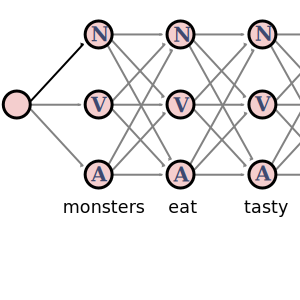
\includegraphics[width=1.5in]{figs/perc_dotprojection}}
  Given two vectors $\vec u$ and $\vec v$ their dot product $\dotp{\vec u}{\vec v}$ is $\sum_d u_d v_d$.
  The dot product grows large and positive when $\vec u$ and $\vec v$ point in same direction, grows
  %\begin{wrapfigure}{r}{2in}
  %  \vspace{-3em}
  %  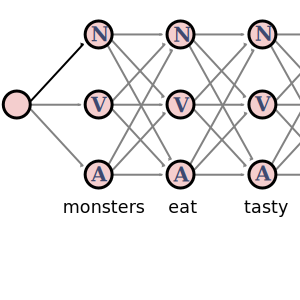
\includegraphics[width=2in]{figs/perc_dotprojection}.
  %\end{wrapfigure}
  large and negative when $\vec u$ and $\vec v$ point in opposite directions, and is zero when their are perpendicular.
  A useful geometric interpretation of dot products is \concept{projection}.
  Suppose $\norm{\vec u} = 1$, so that $\vec u$ is a \concept{unit vector}.
  We can think of any other vector $\vec v$ as consisting of two components: (a) a component in the direction of $\vec u$ and (b) a component that's perpendicular to $\vec u$.
  This is depicted geometrically to the right:
  Here, $\vec u = \langle 0.8, 0.6 \rangle$ and $\vec v = \langle 0.37, 0.73 \rangle$.
  We can think of $\vec v$ as the sum of two vectors, $\vec a$ and $\vec b$, where
  $\vec a$ is parallel to $\vec u$ and $\vec b$ is perpendicular.
  The length of $\vec b$ is exactly $\dotp{\vec u}{\vec v} = 0.734$, which is why you can think of
  dot products as projections: the dot product between $\vec u$ and $\vec v$ is the ``projection of $\vec v$ onto $\vec u$.''
%u=(0.8,0.6) --> (240,180) by *300
%v=(0.37,0.73) --> (110,220) by *300
\end{mathreview}

A question you should be asking yourself by now is: what does the
decision boundary of a perceptron look like?  You can actually answer
that question mathematically.  For a perceptron, the decision boundary
is precisely where the sign of the activation, $a$, changes from $-1$
to $+1$.  In other words, it is the set of points $\vx$ that achieve
\emph{zero} activation.  The points that are not clearly positive nor
negative.  For simplicity, we'll first consider the case where there
is no ``bias'' term (or, equivalently, the bias is zero).  Formally,
the decision boundary $\cB$ is:
\begin{equation}
\cB = \left\{ \vx ~:~ \sum_d w_d x_d = 0 \right\}
\end{equation}
We can now apply some linear algebra.  Recall that $\sum_d w_d x_d$ is
just the \concept{dot product} between the vector $\vw = \langle w_1,
w_2, \dots, w_D \rangle$ and the vector $\vx$.  We will write this as
$\dotp{\vw}{\vx}$.  Two vectors have a zero dot product if and only if
they are \concept{perpendicular}.  Thus, if we think of the weights as
a vector $\vw$, then the decision boundary is simply the plane
perpendicular to $\vw$.

\MoveNextFigure{-1cm}
\Figure{perc:geom}{picture of data points with hyperplane and weight vector}

This is shown pictorially in Figure~\ref{fig:perc:geom}.  Here, the
weight vector is shown, together with it's perpendicular plane.  This
plane forms the decision boundary between positive points and negative
points.  The vector points in the direction of the positive examples
and away from the negative examples.

One thing to notice is that the \emph{scale} of the weight vector is
irrelevant from the perspective of classification.  Suppose you take a
weight vector $\vw$ and replace it with $2 \vw$.  All activations are
now doubled.  But their sign does not change.  This makes complete
sense geometrically, since all that matters is which side of the plane
a test point falls on, now how far it is from that plane.  For this
reason, it is common to work with \koncept{normalized}{normalize}
weight vectors, $\vw$, that have length one; i.e., $\norm{\vw} = 1$.

\thinkaboutit{If I give you a non-zero weight vector $\vw$,
  how do I compute a weight vector $\vw'$ that points in the same
  direction but has a norm of one?}

\MoveNextFigure{-2cm}
\Figure{perc:proj}{The same picture as before, but with projections onto
  weight vector; then, below, those points along a
  one-dimensional axis with zero marked.}

The geometric intuition can help us even more when we realize that
dot products compute projections.  That is, the value $\dotp{\vw}{\vx}$
is just the distance of $\vx$ from the origin when projected
\emph{onto} the vector $\vw$.  This is shown in
Figure~\ref{fig:perc:proj}.  In that figure, all the data points are
projected onto $\vw$.  Below, we can think of this as a
one-dimensional version of the data, where each data point is placed
according to its projection along $\vw$.  This distance along $\vw$ is
exactly the \emph{activiation} of that example, with no bias.

From here, you can start thinking about the role of the bias term.
Previously, the threshold would be at zero.  Any example with a
negative projection onto $\vw$ would be classified negative; any
example with a positive projection, positive.  The bias simply moves
this threshold.  Now, after the projection is computed, $b$ is added
to get the overall activation.  The projection \emph{plus} $b$ is then
compared against zero.

\TODOFigure{perc:bias}{perceptron picture with bias}

Thus, from a geometric perspective, the role of the bias is to
\emph{shift} the decision boundary away from the origin, in the
direction of $\vw$.  It is shifted exactly $-b$ units.  So if $b$ is
positive, the boundary is shifted away from $\vw$ and if $b$ is
negative, the boundary is shifted toward $\vw$.  This is shown in
Figure~\ref{fig:perc:bias}.  This makes intuitive sense: a positive
bias means that more examples should be classified positive.  By
moving the decision boundary in the negative direction, more space
yields a positive classification.

The decision boundary for a perceptron is a very magical thing.  In
$D$ dimensional space, it is always a $D-1$-dimensional hyperplane.
(In two dimensions, a 1-d hyperplane is simply a line.  In three
dimensions, a 2-d hyperplane is like a sheet of paper.)  This
hyperplane divides space in half.  In the rest of this book, we'll
refer to the weight vector, and to hyperplane it defines,
interchangeably.

\Figure{perc:update}{perceptron picture with update, no bias}

The perceptron update can also be considered geometrically.  (For
simplicity, we will consider the \concept{unbiased} case.)  Consider
the situation in Figure~\ref{fig:perc:update}.  Here, we have a current
guess as to the hyperplane, and positive training example comes in
that is currently mis-classified.  The weights are updated: $\vw
\leftarrow \vw + y \vx$.  This yields the new weight vector, also
shown in the Figure.  In this case, the weight vector changed enough
that this training example is now correctly classified.

\section{Interpreting Perceptron Weights}

You may find yourself having run the perceptron, learned a really awesome classifier, and then wondering ``what the heck is this classifier doing?''
You might ask this question because you're curious to learn something about the underlying data.
You might ask this question because you want to make sure that the perceptron is learning ``the right thing.''
You might ask this question because you want to remove a bunch of features that aren't very useful because they're expensive to compute or take a lot of storage.

The perceptron learns a classifier of the form $\vx \mapsto \sign\left( \sum_d w_d x_d + b \right)$.
A reasonable question to ask is: how sensitive is the final classification to \emph{small changes} in some particular feature.
We can answer this question by taking a derivative.
If we arbitrarily take the $7$th feature we can compute $\frac \partial {\partial x_7} \left( \sum_d w_d x_d + b \right) = w_7$.
This says: the rate at which the activation changes as a function of the $7$th feature is exactly $w_7$.
This gives rise to a useful heuristic for interpreting perceptron weights:
\textbf{sort all the weights from largest (positive) to largest (negative), and take the top ten and bottom ten}.
The top ten are the features that the perceptron is most sensitive to for making positive predictions.
The bottom ten are the features that the perceptron is most sensitive to for making negative predictions.

This heuristic is useful, especially when the inputs $\vx$ consist entirely of binary values (like a bag of words representation).
The heuristic is less useful when the range of the individual features varies significantly.
The issue is that if you have one feat $x_5$ that's either $0$ or $1$, and another feature $x_7$ that's either $0$ or $100$, but $w_5 = w_7$, it's reasonable to say that $w_7$ is more important because it is likely to have a much larger influence on the final prediction.
The easiest way to compensate for this is simply to scale your features ahead of time:
this is another reason why feature scaling is a useful preprocessing step.


\section{Perceptron Convergence and Linear Separability}

You already have an intuitive feeling for why the perceptron works: it
moves the decision boundary in the direction of the training
examples.  A question you should be asking yourself is: does the
perceptron converge?  If so, what does it converge to?  And how long
does it take?

It is easy to construct data sets on which the perceptron algorithm
will never converge.  In fact, consider the (very uninteresting)
learning problem with \emph{no features}.  You have a data set
consisting of one positive example and one negative example.  Since
there are no features, the only thing the perceptron algorithm will
ever do is adjust the bias.  Given this data, you can run the
perceptron for a bajillion iterations and it will never settle down.
As long as the bias is non-negative, the negative example will cause
it to decrease.  As long as it is non-positive, the positive example
will cause it to increase.  Ad infinitum.  (Yes, this is a very
contrived example.)

\Figure{perc:separable}{separable data}

What does it mean for the perceptron to converge?  It means that it
can make an entire pass through the training data without making
\emph{any} more updates.  In other words, it has correctly classified
\emph{every} training example.  Geometrically, this means that it was
found some hyperplane that correctly segregates the data into positive
and negative examples, like that shown in
Figure~\ref{fig:perc:separable}.

\Figure{perc:inseparable}{inseparable data}

In this case, this data is \concept{linearly separable}.  This means
that there exists \emph{some} hyperplane that puts all the positive
examples on one side and all the negative examples on the other side.
If the training is \emph{not} linearly separable, like that shown in
Figure~\ref{fig:perc:inseparable}, then the perceptron has no hope of
converging.  It could never possibly classify each point correctly.

The somewhat surprising thing about the perceptron algorithm is that
\emph{if} the data is linearly separable, \emph{then} it will converge
to a weight vector that separates the data.  (And if the data is
inseparable, then it will never converge.)  This is great news.  It
means that the perceptron converges whenever it is even remotely
possible to converge.

The second question is: how long does it take to converge?  By ``how
long,'' what we really mean is ``how many updates?''  As is the case
for much learning theory, you will not be able to get an answer of the
form ``it will converge after $5293$ updates.''  This is asking too
much.  The sort of answer we can hope to get is of the form ``it will
converge after \emph{at most} $5293$ updates.''

What you might expect to see is that the perceptron will converge more
quickly for easy learning problems than for hard learning problems.
This certainly fits intuition.  The question is how to \emph{define}
``easy'' and ``hard'' in a meaningful way.  One way to make this
definition is through the notion of \concept{margin}.  If I give you a
data set and hyperplane that separates it% (like that shown in
%Figure~\ref{fig:perc:margin}) 
then the \emph{margin} is the distance
between the hyperplane and the nearest point.  Intuitively, problems
with large margins should be easy (there's lots of ``wiggle room'' to
find a separating hyperplane); and problems with small margins should
be hard (you really have to get a very specific well tuned weight
vector).

Formally, given a data set $\mat D$, a weight vector $\vw$ and bias
$b$, the margin of $\vw,b$ on $\mat D$ is defined as:
\begin{equation} \label{eq:margin}
\textit{margin}(\mat D, \vw, b)
= \brack{
     \min_{(\vx,y) \in \mat D} y \big( \dotp{\vw}{\vx} + b \big)
      & \text{if $\vw$ separates $\mat D$} \\
    -\infty & \text{otherwise}
}
\end{equation}
In words, the margin is only defined if $\vw,b$ actually separate the
data (otherwise it is just $-\infty$).  In the case that it separates
the data, we find the point with the minimum activation, after the
activation is multiplied by the label.
\thinkaboutit{So long as the margin is not $-\infty$, it is always
  positive.  Geometrically this makes sense, but why does
  Eq~\eqref{eq:margin} yield this?}

For some historical reason (that is unknown to the author), margins
are always denoted by the Greek letter $\gamma$ (gamma).  One often
talks about the \concept{margin of a data set}.  The margin of a data
set is the largest attainable margin on this data.  Formally:
\begin{equation} \label{eq:margin2}
\textit{margin}(\mat D)
= 
\sup_{\vw,b} \textit{margin}(\mat D, \vw, b)
\end{equation}
In words, to compute the margin of a data set, you ``try'' every
possible $\vw,b$ pair.  For each pair, you compute its margin.  We
then take the largest of these as the overall margin of the
data.\sidenote{You can read ``$\sup$'' as ``$\max$'' if you like: the
  only difference is a technical difference in how the $-\infty$ case
  is handled.}  If the data is not linearly separable, then the value
of the $\sup$, and therefore the value of the margin, is $-\infty$.

There is a famous theorem due to
Rosenblatt\mycite{rosenblatt58perceptron} that shows that the number
of errors that the perceptron algorithm makes is bounded by
$\ga^{-2}$.  More formally:

\begin{theorem}[Perceptron Convergence Theorem] \label{thm:perc:perc}
  Suppose the perceptron algorithm is run on a linearly separable data
  set $\mat D$ with margin $\ga > 0$.  Assume that $\norm{\vx} \leq 1$
  for all $\vx \in \mat D$.  Then the algorithm will converge after at
  most $\frac 1 {\ga^2}$ updates.
\end{theorem}

The proof of this theorem is elementary, in the sense that it does not
use any fancy tricks: it's all just algebra.  The \emph{idea} behind
the proof is as follows.  If the data is linearly separable with
margin $\ga$, then there exists some weight vector $\vw^*$ that
achieves this margin.  Obviously we don't know what $\vw^*$ is, but we
know it exists.  The perceptron algorithm is trying to find a weight
vector $\vw$ that points roughly in the same direction as $\vw^*$.
(For large $\ga$, ``roughly'' can be very rough.  For small $\ga$,
``roughly'' is quite precise.)  Every time the perceptron makes an
update, the angle between $\vw$ and $\vw^*$ changes.  What we prove is
that the angle actually \emph{decreases.}  We show this in two steps.
First, the dot product $\dotp{\vw}{\vw^*}$ increases a lot.  Second,
the norm $\norm{\vw}$ does not increase very much.  Since the dot
product is increasing, but $\vw$ isn't getting too long, the angle
between them has to be shrinking.  The rest is algebra.

\begin{myproof}{\ref{thm:perc:perc}}
  The margin $\ga > 0$ must be realized by some set of parameters, say
  $\vx^*$.  Suppose we train a perceptron on this data.  Denote by
  $\vw\zth$ the initial weight vector, $\vw\oth$ the weight vector
  after the \emph{first update}, and $\vw\kth$ the weight vector after
  the $k$th update.  (We are essentially ignoring data points on which
  the perceptron doesn't update itself.)  First, we will show that
  $\dotp{\vw^*}{\vw\kth}$ grows quicky as a function of $k$.  Second,
  we will show that $\norm{\vw\kth}$ does not grow quickly.

  First, suppose that the $k$th update happens on example $(\vx,y)$.
  We are trying to show that $\vw\kth$ is becoming aligned with
  $\vw^*$.  Because we updated, know that this example was
  misclassified: $y \dotp{\vw\kpth}{\vx} < 0$.  After the update, we get
  $\vw\kth = \vw\kpth + y \vx$.  We do a little computation:
  \begin{align}
    \dotp{\vw^*}{\vw\kth}
    &= \dotp{\vw^*}{\left(\vw\kpth + y \vx\right)} 
         \becauseof{definition of $\vw\kth$}
    \\
    &= \dotp{\vw^*}{\vw\kpth} + y \dotp{\vw^*}{\vx}
         \becauseof{vector algebra}
    \\
    &\geq \dotp{\vw^*}{\vw\kpth} + \ga
         \becauseof{$\vw^*$ has margin $\ga$}
  \end{align}
  Thus, every time $\vw\kth$ is updated, its projection onto $\vw^*$
  increases by at least $\ga$.  \textcolor{darkblue}{Therefore:
    $\dotp{\vw^*}{\vw\kth} \geq k \ga$.}

  Next, we need to show that the increase of $\ga$ along $\vw^*$
  occurs because $\vw\kth$ is getting closer to $\vw^*$, not just
  because it's getting exceptionally long.  To do this, we compute the
  norm of $\vw\kth$:
  \begin{align}
    & \norm{\vw\kth}^2 \nonumber\\
    &= \norm{\vw\kpth + y \vx}^2
         \becauseof{def. of $\vw\kth$} \\
    &= \norm{\vw\kpth}^2 + y^2 \norm{\vx}^2 + 2 y \dotp{\vw\kpth}{\vx}
         \becauseof{quadratic rule} \\
    &\leq \norm{\vw\kpth}^2 + 1 + 0
         \becauseof{assumption and $a < 0$}
  \end{align}
  Thus, the squared norm of $\vw\kth$ increases by at most one every
  update.  \textcolor{darkblue}{Therefore: $\norm{\vw\kth}^2 \leq k$.}

  Now we put together the two things we have learned before.  By our
  first conclusion, we know $\dotp{\vw^*}{\vw\kth} \geq k \ga$.  But
  our second conclusion, $\sqrt{k} \geq \norm{\vw\kth}^2$.  Finally,
  because $\vw^*$ is a unit vector, we know that $\norm{\vw\kth} \geq
  \dotp{\vw^*}{\vw\kth}$.  Putting this together, we have:
  \begin{equation}
    \sqrt k 
    \quad\geq\quad
    \norm{\vw\kth}
    \quad\geq\quad
    \dotp{\vw^*}{\vw\kth}
    \quad\geq\quad
    k\ga
  \end{equation}
  Taking the left-most and right-most terms, we get that $\sqrt{k}
  \geq k \ga$.  Dividing both sides by $k$, we get $\frac 1 {\sqrt{k}}
  \geq \ga$ and therefore $k \leq \frac 1 {\ga^2}$.  This means
  that once we've made $\frac 1 {\ga^2}$ updates, we cannot make
  any more!
\end{myproof}

\thinkaboutit{Perhaps we don't want to assume that all $\vx$ have norm
  at most $1$.  If they have all have norm at most $R$, you can
  achieve a very similar bound.  Modify the perceptron convergence
  proof to handle this case.}


It is important to keep in mind what this proof shows and what it does
not show.  It shows that if I give the perceptron data that is
linearly separable with margin $\gamma > 0$, then the perceptron will
converge to a solution that separates the data.  And it will converge
quickly when $\gamma$ is large.  It does not say anything about the
solution, \emph{other than} the fact that it separates the data.  In
particular, the proof makes use of the maximum margin separator.  But
the perceptron is not guaranteed to \emph{find} this maximum margin
separator.  The data may be separable with margin $0.9$ and the
perceptron might still find a separating hyperplane with a margin of
only $0.000001$.  Later (in Chapter~\ref{sec:loss}), we will see
algorithms that explicitly try to find the maximum margin solution.

\thinkaboutit{Why does the perceptron convergence bound not contradict
  the earlier claim that poorly ordered data points (e.g., all
  positives followed by all negatives) will cause the perceptron to
  take an astronomically long time to learn?}

\section{Improved Generalization: Voting and Averaging}

In the beginning of this chapter, there was a comment that the
perceptron works amazingly well.  This was a half-truth.  The
``vanilla'' perceptron algorithm does well, but not \emph{amazingly}
well.  In order to make it more competitive with other learning
algorithms, you need to modify it a bit to get better generalization.
The key issue with the vanilla perceptron is that \emph{it counts
  later points more than it counts earlier points}.

To see why, consider a data set with $10,000$ examples.  Suppose that
after the first $100$ examples, the perceptron has learned a really
good classifier.  It's so good that it goes over the next $9899$
examples without making \emph{any} updates.  It reaches the $10,000$th
example and makes an error.  It updates.  For all we know, the update
on this $10,000$th example \emph{completely ruins} the weight vector
that has done so well on $99.99\%$ of the data!

What we would like is for weight vectors that ``survive'' a long time
to get more say than weight vectors that are overthrown quickly.  One
way to achieve this is by \concept{voting}.  As the perceptron learns,
it remembers how long each hyperplane survives.  At test time, each
hyperplane encountered during training ``votes'' on the class of a
test example.  If a particular hyperplane survived for $20$ examples,
then it gets a vote of $20$.  If it only survived for one example, it
only gets a vote of $1$.  In particular, let $(\vw,b)\oth, \dots,
(\vw,b)\Kth$ be the $K+1$ weight vectors encountered during training,
and $c\oth, \dots, c\Kth$ be the survival times for each of these
weight vectors.  (A weight vector that gets immediately updated gets
$c=1$; one that survives another round gets $c=2$ and so on.)  Then
the prediction on a test point is:
\begin{equation} \label{eq:perc:vote}
  \hat y = \sign \left(
    \sum_{k=1}^K c\kth 
      \sign \left(
        \dotp{\vw\kth}{\hat\vx} + b\kth
        \right)
      \right)
\end{equation}
This algorithm, known as the \concept{voted perceptron} works quite
well in practice, and there is some nice theory showing that it is
guaranteed to generalize better than the vanilla perceptron.
Unfortunately, it is also completely impractical.  If there are $1000$
updates made during perceptron learning, the voted perceptron requires
that you store $1000$ weight vectors, together with their counts.
This requires an absurd amount of storage, and makes prediction $1000$
times slower than the vanilla perceptron.

\thinkaboutit{The \emph{training algorithm} for the voted perceptron
  is the same as the vanilla perceptron.  In particular, in line 5 of
  Algorithm~\ref{alg:perc:perc}, the activation on a training example
  is computed based on the \emph{current weight vector}, not based on
  the voted prediction.  Why?}

A much more practical alternative is the \concept{averaged
  perceptron}.  The idea is similar: you maintain a collection of
weight vectors and survival times.  However, at test time, you predict
according to the \emph{average} weight vector, rather than the
voting.  In particular, the prediction is:
\begin{equation} \label{eq:perc:avg}
  \hat y = \sign \left(
    \sum_{k=1}^K c\kth 
      \left(
        \dotp{\vw\kth}{\hat\vx} + b\kth
        \right)
      \right)
\end{equation}
The only difference between the voted prediction,
Eq~\eqref{eq:perc:vote}, and the averaged prediction,
Eq~\eqref{eq:perc:avg}, is the presense of the interior $\sign$
operator.  With a little bit of algebra, we can rewrite the test-time
prediction as:
\begin{equation}
  \hat y = \sign \left(
    \dotp{\textcolor{darkblue}{\left(
        \sum_{k=1}^K c\kth \vw\kth 
        \right)}}{\hat\vx} +
      \textcolor{darkred}{\sum_{k=1}^K c\kth b\kth}
      \right)
\end{equation}
The advantage of the averaged perceptron is that we can simply
maintain a \emph{running sum} of the averaged weight vector (the blue
term) and averaged bias (the red term).  Test-time prediction is then
just as efficient as it is with the vanilla perceptron.

\newalgorithm%
  {perc:avgperc}%
  {\FUN{AveragedPerceptronTrain}(\VAR{$\mat D$}, \VAR{MaxIter})}
  {
\SETST{$\vw$}{$\langle \CON{0}, \CON{0}, \dots \CON{0} \rangle$
  \quad,\quad
  \VAR{$b$} $\leftarrow$ \CON{0}}
  \COMMENT{initialize weights and bias}
\SETST{$\vec u$}{$\langle \CON{0}, \CON{0}, \dots \CON{0} \rangle$
  \quad,\quad
  \VAR{$\beta$} $\leftarrow$ \CON{0}}
  \COMMENT{initialize cached weights and bias}
\SETST{c}{\CON{1}}
  \COMMENT{initialize example counter to one}
\FOR{\VAR{iter} = \CON{1} \dots \VAR{MaxIter}}
\FORALL{(\VAR{$\vx$},\VAR{$y$}) $\in$ \VAR{$\mat D$}}
\IF{\VAR{$y$}$\left( \dotp{\VARm{\vw}}{\VARm{\vx}} + \VARm{b} \right) \leq \CON{0}$}
\SETST{$\vw$}{\VAR{$\vw$} + \VAR{$y$} \VAR{$\vx$}}
  \COMMENT{update weights}
\SETST{$b$}{\VAR{$b$} + \VAR{$y$}}
  \COMMENT{update bias}
\SETST{$\vec u$}{\VAR{$\vec u$} + \VAR{$y$} \VAR{c} \VAR{$\vx$}}
  \COMMENT{update cached weights}
\SETST{$\beta$}{\VAR{$\beta$} + \VAR{$y$} \VAR{c}}
  \COMMENT{update cached bias}
\ENDIF
\SETST{c}{\VAR{c} + \CON{1}}
  \COMMENT{increment counter regardless of update}
\ENDFOR
\ENDFOR
\RETURN \VAR{$\vw$} - $\frac 1 {\VAR{c}}$ \VAR{$\vec u$}, 
        \VAR{$b$}   - $\frac 1 {\VAR{c}}$ \VAR{$\beta$}
\COMMENT{return averaged weights and bias}
}

The full training algorithm for the averaged perceptron is shown in
Algorithm~\ref{alg:perc:avgperc}.  Some of the notation is changed
from the original perceptron: namely, vector operations are written as
vector operations, and the activation computation is folded into the
error checking.

It is probably not immediately apparent from
Algorithm~\ref{alg:perc:avgperc} that the computation unfolding is
precisely the calculation of the averaged weights and bias.  The most
\emph{natural} implementation would be to keep track of an averaged
weight vector $\vec u$.  At the end of every example, you would
increase $\vec u \leftarrow \vec u + \vw$ (and similarly for the
bias).  However, such an implementation would require that you updated
the averaged vector on \emph{every} example, rather than just on the
examples that were incorrectly classified!  Since we hope that
eventually the perceptron learns to do a good job, we would hope that
it will not make updates on every example.  So, ideally, you would
like to only update the averaged weight vector when the actual weight
vector changes.  The slightly clever computation in
Algorithm~\ref{alg:perc:avgperc} achieves this.

\thinkaboutit{By writing out the computation of the averaged weights
  from Eq~\eqref{eq:perc:avg} as a telescoping sum, derive the
  computation from Algorithm~\ref{alg:perc:avgperc}.}

%\TODOFigure{perc:avgperc}{train/test performance of vanilla versus
%  averaged perceptron to show early stopping}

The averaged perceptron is almost always better than the perceptron,
in the sense that it generalizes better to test data.  However, that
does not free you from having to do \concept{early stopping}.  It
will, eventually, overfit.  
%Figure~\ref{fig:perc:avgperc} shows the
%performance of the vanilla perceptron and the averaged perceptron on
%the same data set, with both training and test performance.  As you
%can see, the averaged perceptron \emph{does} generalize better.  But
%it also does begin to overfit eventually.

\section{Limitations of the Perceptron}


Although the perceptron is very useful, it is fundamentally limited in
a way that neither decision trees nor KNN are.  Its limitation is that
its decision boundaries can \emph{only} be linear.  The classic way of
showing this limitation is through the XOR problem (XOR = exclusive
or).  The XOR problem is shown graphically in
Figure~\ref{fig:perc:xor}.  It consists of four data points, each at a
corner of the unit square.  The labels for these points are the same,
along the diagonals.  You can try, but you will not be able to find a
linear decision boundary that perfectly separates these data points.

\Figure{perc:xor}{picture of xor problem}

One question you might ask is: do XOR-like problems exist in the real
world?  Unfortunately for the perceptron, the answer is yes.  Consider
a sentiment classification problem that has three features that simply
say whether a given word is contained in a review of a course.  These
features are: \feat{excellent}, \feat{terrible} and \feat{not}.  The
\feat{excellent} feature is indicative of positive reviews and the
\feat{terrible} feature is indicative of negative reviews.  But in the
presence of the \feat{not} feature, this categorization flips.

One way to address this problem is by adding \concept{feature
  combinations}.  We could add two additional features:
\feat{excellent-and-not} and \feat{terrible-and-not} that indicate
a conjunction of these base features.  By assigning weights as
follows, you can achieve the desired effect:
\begin{align*}
w_{\feat{execellent}} &= +1
& w_{\feat{terrible}} &= -1
& w_{\feat{not}} &= 0 \\
w_{\feat{execllent-and-not}} &= -2 
& w_{\feat{terrible-and-not}} &= +2
\end{align*}
In this particular case, we have addressed the problem.  However, if
we start with $D$-many features, if we want to add all pairs, we'll
blow up to ${D \choose 2} = \cO(D^2)$ features through this
\concept{feature mapping}.  And there's no guarantee that pairs of
features is enough.  We might need triples of features, and now we're
up to ${D \choose 3} = \cO(D^2)$ features.  These additional features
will drastically increase computation and will often result in a
stronger propensity to overfitting.

\thinkaboutit{Suppose that you took the XOR problem and added one new
  feature: $x_3 = x_1 \land x_2$ (the logical and of the two existing
  features).  Write out feature weights and a bias that would achieve
  perfect classification on this data.}

In fact, the ``XOR problem'' is so significant that it basically
killed research in classifiers with linear decision boundaries for a
decade or two.  Later in this book, we will see two alternative
approaches to taking key ideas from the perceptron and generating
classifiers with non-linear decision boundaries.  One approach is to
combine multiple perceptrons in a single framework: this is the
\concept{neural networks} approach (see Chapter~\ref{sec:nnet}).  The
second approach is to find computationally efficient ways of doing
feature mapping in a computationally and statistically efficient way:
this is the \concept{kernels} approach (see Chapter~\ref{sec:kernel}).

% \TODOFigure{perc:mapping}{mapping two dimensional data, three points,
%   into five dimensional data}

% In addition to the perceptron not being able to \emph{solve} problems
% that require non-linear decision boundaries, it will not even
% \emph{converge} on such problems.  However, there is a simple data
% transformation that ensures linear separability.  Suppose you start
% $N$ training examples in $D$ dimensions.  You will end up with $N$
% training examples in $D+N$ dimensions.  When we map data point $\vx_n
% \mapsto \vx'_n$, you will \emph{copy} the first $D$ dimensions.  After
% those original $D$ dimension, you place an \emph{indicator} in the
% $D+n$th position and zeros everywhere else.
% Figure~\ref{fig:perc:mapping} shows an example on a very small
% training set.

% \thinkaboutit{Completely ignoring the first $D$ many features,
%   construct a weight vector that achieves perfect classification on
%   this data.}

% In practice, there is little reason to \emph{actually} perform this
% mapping.  It is more interesting from a theoretical perspective.  

\section{Further Reading}

TODO further reading


\begin{comment}
   -``Neural network'' interpretation
   - Update rule
   - Linear decision boundaries
   - Connection to geometry, linear algebra, dot products, etc.
   - Linear separability and the XOR problem
   - Margins
   - Convergence
\end{comment}


%%% Local Variables: 
%%% mode: latex
%%% TeX-master: "courseml"
%%% End: 

